\chapter{Budowa aplikacji do zbierania danych badawczych}

Zbieranie danych badawczych jest kluczowym elementem wielu projektów naukowych i biznesowych. Aby ułatwić ten proces, postanowiłem stworzyć aplikację, która pozwoli na efektywne i systematyczne gromadzenie informacji. W tym rozdziale opiszę, jak zbudowałem tę aplikację, składającą się z dwóch głównych komponentów: backendu i frontendu.

\section{Backend}

Backend aplikacji został zbudowany z użyciem języka Java oraz frameworka Spring Boot, który był niezbędny do utworzenia aplikacji webowej i wspomagał routing.
Do utworzonego projektu najpierw zaimportowałem bibliotekę Lombok oraz narzędzie Liquibase do sprawnego korzystania z baz danych, poprzez zależności:
\begin{lstlisting}
<dependency>
    <groupId>org.projectlombok</groupId>
    <artifactId>lombok</artifactId>
</dependency>
<dependency>
    <groupId>org.liquibase</groupId>
    <artifactId>liquibase-core</artifactId>
    <version>4.20.0</version>
</dependency>      
\end{lstlisting}

Następnie zająłem się utworzeniem połączenie do bazy danych Oracle poprzez dodanie odpowiedniej zależności dla Mavena:
\begin{lstlisting}
<dependency>
   <groupId>com.oracle.database.jdbc</groupId>
   <artifactId>ojdbc8</artifactId>
   <version>21.9.0.0</version>
</dependency>
\end{lstlisting}
Po uwzględnieniu zależności ustawiłem konfigurację w \textit{application.properties} dla mojego podłączenia do bazy danych, która powinna wyglądać następująco:

\begin{lstlisting}
spring.liquibase.change-log=classpath:/db/changelog/db.changelog-master.xml
spring.liquibase.contexts=development
spring.datasource.url=jdbc:oracle:thin:@10.169.168.5:1521:xe
spring.datasource.username=C##AWMED
spring.datasource.password=pzespol
spring.datasource.driver-class-name=oracle.jdbc.OracleDriver

spring.jpa.database-platform=org.hibernate.dialect.Oracle12cDialect
spring.jpa.hibernate.ddl-auto=update
firebase.config.path=key.json
\end{lstlisting}

W ten sposób uzyskałem pełne podłączenie do jednej z dwóch baz danych potrzebnych do testów wydajności. Kolejnym krokiem było podłączenie bazy Firebase od Google, czyli dodanie kolejnej zależności:

\begin{lstlisting}
<dependency>
   <groupId>com.google.firebase</groupId>
   <artifactId>firebase-admin</artifactId>
   <version>9.2.0</version>
</dependency>
\end{lstlisting}

Po dodaniu zależności należało utworzyć klasę konfiguracyjną w kodzie, która będzie pozwalała na ustanowienie połączenia z Firebase oraz pobieranie i wysyłanie danych na serwer.
Tą klasą jest \textit{FirebaseConfig} z odpowiednią adnotacją \textit{@Configration} powodującą zainicjalizowanie tej klasy przy uruchomieniu aplikacji.
Klasa ta wygląda następująco:
\begin{lstlisting}
package org.example.service;

import com.google.api.core.ApiFuture;
import com.google.auth.oauth2.GoogleCredentials;
import com.google.cloud.firestore.CollectionReference;
import com.google.cloud.firestore.DocumentReference;
import com.google.cloud.firestore.Firestore;
import com.google.firebase.FirebaseApp;
import com.google.firebase.FirebaseOptions;

import com.google.firebase.cloud.FirestoreClient;
import com.google.firebase.database.*;
import org.example.FireBaseApi;
import org.example.GameApi;
import org.springframework.context.annotation.Bean;
import org.springframework.context.annotation.Configuration;

import java.io.IOException;
import java.io.InputStream;
import java.util.ArrayList;
import java.util.List;
import java.util.concurrent.ExecutionException;

@Configuration
public class FirebaseConfig {


    @Bean
    public FirebaseApp firebaseApp() throws IOException {
        InputStream refreshToken = getClass().getResourceAsStream("/key.json");
        FirebaseOptions options = FirebaseOptions.builder()
                .setCredentials(GoogleCredentials.fromStream(refreshToken))
                .setDatabaseUrl("https://databases-3fd9e.firebaseio.com/")
                .build();

        FirebaseApp.initializeApp(options);

        return FirebaseApp.getInstance();
    }

    public List<GameApi> getFromFireBase(){
        List<GameApi> gameApiList = new ArrayList<>();
        DatabaseReference rootRef = FirebaseDatabase.getInstance().getReference();
        rootRef.addListenerForSingleValueEvent(new ValueEventListener() {
            @Override
            public void onDataChange(DataSnapshot dataSnapshot) {
                for(DataSnapshot ds : dataSnapshot.getChildren()) {
                    GameApi gameApi = ds.getValue(GameApi.class);
                    gameApiList.add(gameApi);
                }
            }

            @Override
            public void onCancelled(DatabaseError error) {
                System.out.println("The read failed: " + error.getCode());
            }
        });
        return gameApiList;
    }

    public void addToFirebase(FireBaseApi gameApi) {
        Firestore firestore = FirestoreClient.getFirestore();
        CollectionReference gamesCollection = firestore.collection("games");

        ApiFuture<DocumentReference> future = gamesCollection.add(gameApi);

        try {
            DocumentReference documentReference = future.get();
            System.out.println("Game added to Firestore successfully at: " + documentReference.getPath());
        } catch (InterruptedException | ExecutionException e) {
            System.out.println("Error adding game to Firestore: " + e.getMessage());
        }
    }
}
\end{lstlisting}
\begin{itemize}
\item \textit{firebaseApp()} -- metoda inicjalizująca połączenie z bazą Firebase, wywołuje klasę \textit{FirebaseOptions}, która po ustawieniu odpowiednich ,,credentials'' oraz ,,databaseUrl'' odnoszącego się do adresu mojej bazy tworzy połączenie i zwraca instację tego połączenia.

\item \textit{getFromFireBase()} -- metoda pozwalająca na pobranie obiektów z bazy danych, wołana później w momencie uzyskiwania rekordów dla użytkownika, co będzie omawiane w dalszej części rozdziału

\item \textit{addToFireBase()} -- metoda pozwalająca na dodawanie rekordów do bazy danych, klasa \textit{CollectionRefference} pozwalała na określenie katalogu dla konkretnych rekordów 
\end{itemize}

Na tym etapie, w aplikacji jest już połączenie do bazy obu baz danych oraz zaimportowane potrzebne zależności. Skupiłem się więc na tworzeniu modelu API gry, która będzie przechowywana na bazie oraz zwracana do wyświetlenia u użytkownika. Model ten wygląda następująco:
\begin{lstlisting}
public class GameApi {
    private Long id;
    private String gameName;
    private String gameType;
    private String multiplayer;
    private String platform;
    private Long age;
    private String wydawca;
    private LocalDate dateOfOut;
    private String transactions;
    private String motyw;
    private String description;
    private Long ranking;
}
\end{lstlisting}

Aby poprawnie dodać obiekt do Firebase, daty powinny być zapisywane w formacie \textit{String}, przez co utworzyłem dedykowany model API dla Firebase, który posiadał zmieniony format dat.

Po ustaleniu odpowiedniego API skupiłem się na utworzeniu tabeli w bazie Oracle przy użyciu liquibase. Liquibase jest zapisany w formacie \textit{XML} i wygląda następująco:
\begin{lstlisting}
<?xml version="1.0" encoding="UTF-8"?>
<databaseChangeLog
        xmlns="http://www.liquibase.org/xml/ns/dbchangelog"
        xmlns:xsi="http://www.w3.org/2001/XMLSchema-instance"
        xsi:schemaLocation="http://www.liquibase.org/xml/ns/dbchangelog
         http://www.liquibase.org/xml/ns/dbchangelog/dbchangelog-3.8.xsd">

    <changeSet id="GAMES_LIST_TABLE" author="adam.wadowski">
        <preConditions onFail="MARK_RAN">
            <not>
                <tableExists tableName="games_list"/>
            </not>
        </preConditions>
        <createTable tableName="games_list">
            <column name="id" type="number">
                <constraints nullable="false" unique="true"/>
            </column>
            <column name="game_type" type="varchar2(255)">
                <constraints nullable="true"/>
            </column>
            <column name="game_name" type="varchar2(255)">
                <constraints nullable="true"/>
            </column>
            <column name="multiplayer" type="varchar2(2)">
                <constraints nullable="true"/>
            </column>
            <column name="platform" type="varchar2(255)">
                <constraints nullable="true"/>
            </column>
            <column name="age" type="number">
                <constraints nullable="true"/>
            </column>
            <column name="wydawca" type="varchar2(255)">
                <constraints nullable="true"/>
            </column>
            <column name="date_of_out" type="date">
                <constraints nullable="true"/>
            </column>
            <column name="transactions" type="varchar2(2)">
                <constraints nullable="true"/>
            </column>
            <column name="motyw" type="varchar2(255)">
                <constraints nullable="true"/>
            </column>
        </createTable>
    </changeSet>

    <changeSet id="GAMES_LIST_SEQ" author="adam.wadowski">
        <preConditions onFail="MARK_RAN">
            <not>
                <sequenceExists sequenceName="games_list_id_seq"/>
            </not>
        </preConditions>
        <createSequence sequenceName="games_list_id_seq" startValue="1"/>
    </changeSet>

    <changeSet id="GAMES_LIST_add_description-1" author="adam.wadowski">
        <preConditions onFail="MARK_RAN">
            <not>
                <columnExists columnName="DESCRIPTION" tableName="GAMES_LIST"/>
            </not>
        </preConditions>
        <addColumn tableName="GAMES_LIST">
            <column name="DESCRIPTION" remarks="opis" type="VARCHAR(1500)"></column>
        </addColumn>
    </changeSet>

    <changeSet id="GAMES_LIST_add_ranking-1" author="adam.wadowski">
        <preConditions onFail="MARK_RAN">
            <not>
                <columnExists columnName="ranking" tableName="GAMES_LIST"/>
            </not>
        </preConditions>
        <addColumn tableName="GAMES_LIST">
            <column name="ranking" remarks="ranking" type="number"></column>
        </addColumn>
    </changeSet>

</databaseChangeLog>
\end{lstlisting}

Został jeszcze problem przechowywania wyników dla czasów wyszukiwania poszczególnych baz danych, dlatego utworzyłem również tabelę \textit{SEARCHING}, która zawierała pola takie jak:
\begin{itemize}
\item \textit{searching type} -- typ wyszukiwania, rozróżnienie na wyszukiwanie w bazie Oracle lub Firebase
\item \textit{searching mode} -- czas wyszukiwania podawany w milisekundach
\end{itemize}
Po skonfigurowaniu bazy danych Oracle, utworzyłem ,,controllery'' wystawiające usługi od odczytu przez aplikację frontendową. Jeden controller przyjmuje obiekt GameApi w którym sprecyzowane są wartości do wyszukiwania gier i zwraca listę gier, które spełniają określone kryteria podane przez użytkownika. Wygląda on następująco:
\begin{lstlisting}
@PostMapping("/findByCriteria")
    public List<GameApi> findByCriteria(@RequestBody GameApi gameApi) {
        return gameService.findByCriteria(gameApi);
    }
\end{lstlisting}

Jak widać obsługa tego controllera zapisana jest w gameService i wygląda następująco:
\begin{lstlisting}
 public List<GameApi> findByCriteria(GameApi criteria) {
        List<GameApi> results = findByCriteriaInternal(criteria);
        findFromFirebase(criteria);
        if (results.size()<3) {
            if (criteria.getMotyw() != null) {
                criteria.setMotyw(null);
            } else if (criteria.getTransactions() != null) {
                criteria.setTransactions(null);
            } else if (criteria.getDateOfOut() != null) {
                criteria.setDateOfOut(null);
            } else if (criteria.getWydawca() != null) {
                criteria.setWydawca(null);
            } else if (criteria.getAge() != null) {
                criteria.setAge(null);
            } else if (criteria.getPlatform() != null) {
                criteria.setPlatform(null);
            } else if (criteria.getMultiplayer() != null) {
                criteria.setMultiplayer(null);
            } else if (criteria.getGameType() != null) {
                criteria.setGameType(null);
            }
            return findByCriteria(criteria);
        }
        results.sort((o1, o2) -> o2.getRanking().compareTo(o1.getRanking()));
        return results.subList(0,3);
    }
    
        private List<GameApi> findByCriteriaInternal(GameApi criteria) {
        SearchingEntity searchingEntity = new SearchingEntity();
        searchingEntity.setSearchingType("oracle");
        long startTime = System.nanoTime();
        List<GameEntity> results = new ArrayList<>();
        gameRepository.findAll().forEach(game -> {
            if ((criteria.getGameType() == null || game.getGameType().equals(criteria.getGameType())) &&
                    (criteria.getMultiplayer() == null || game.getMultiplayer().equals(criteria.getMultiplayer())) &&
                    (criteria.getPlatform() == null || game.getPlatform().equals(criteria.getPlatform())) &&
                    (criteria.getAge() == null || game.getAge() <= criteria.getAge()) &&
                    (criteria.getWydawca() == null || game.getWydawca().equals(criteria.getWydawca())) &&
                    (criteria.getDateOfOut() == null || game.getDateOfOut().equals(criteria.getDateOfOut())) &&
                    (criteria.getTransactions() == null || game.getTransactions().equals(criteria.getTransactions())) &&
                    (criteria.getMotyw() == null || game.getMotyw().equals(criteria.getMotyw()))) {
                results.add(game);
            }
        });
        long endTime = System.nanoTime();
        long duration = (endTime - startTime);
        searchingEntity.setSearchingTime(String.valueOf(duration/1_000));
        searchingRepository.save(searchingEntity);
        return gameConverter.fromEntityList(results);
    }

    @Async
    protected void findFromFirebase(GameApi criteria){
        SearchingEntity searchingEntity = new SearchingEntity();
        searchingEntity.setSearchingType("firebase");
        long startTime = System.nanoTime();
        List<GameApi> results = new ArrayList<>();
        firebaseConfig.getFromFireBase().forEach(game -> {
            if ((criteria.getGameType() == null || game.getGameType().equals(criteria.getGameType())) &&
                    (criteria.getMultiplayer() == null || game.getMultiplayer().equals(criteria.getMultiplayer())) &&
                    (criteria.getPlatform() == null || game.getPlatform().equals(criteria.getPlatform())) &&
                    (criteria.getAge() == null || game.getAge() <= criteria.getAge()) &&
                    (criteria.getWydawca() == null || game.getWydawca().equals(criteria.getWydawca())) &&
                    (criteria.getDateOfOut() == null || game.getDateOfOut().equals(criteria.getDateOfOut())) &&
                    (criteria.getTransactions() == null || game.getTransactions().equals(criteria.getTransactions())) &&
                    (criteria.getMotyw() == null || game.getMotyw().equals(criteria.getMotyw()))) {
                results.add(game);
            }
        });
        long endTime = System.nanoTime();
        long duration = (endTime - startTime);
        searchingEntity.setSearchingTime(String.valueOf(duration/1_000));
        searchingRepository.save(searchingEntity);
    }
\end{lstlisting}

Obiekty są wyszukiwane na podstawie podanych kryteriów przez użytkownika w dwóch bazach, jednak zwracana lista jest zwracana tylko z bazy Oracle. Obie metody działają identycznie mierząc czas dla takiej samej operacji, a później zapisując czas do tabeli \textit{SEARCHING} przez co możemy łatwo odczytać wynik jednym zapytaniem.

Drugą usługą wystawioną w \textit{Controllerze} jest usługa do zmiany rankingu danej pozycji, użytkownik po wyszukiwaniu gier, będzie miał możliwość oceny czy gra spełnia jego oczekiwania czy nie, co będzie wpływało na ranking konkretnej gry i skutkowało jej wyświetlaniem w późniejszym etapie. Usługa ta wygląda następująco:
\begin{lstlisting}
    @PutMapping("/changeRanking/{id}/{ranking}")
    public void changeRanking(@PathVariable Long id, @PathVariable Long ranking){
        gameService.changeRanking(id,ranking);
    }
\end{lstlisting}
A w serwisie usługa prezentuje się w następujący sposób:
\begin{lstlisting}
    public void changeRanking(Long id, Long ranking){
        GameEntity gameEntity = gameRepository.findById(id).orElseThrow(() -> new RuntimeException("Nie znaleziono gry o podanym id"));
        gameEntity.setRanking(ranking);
        gameRepository.save(gameEntity);
    }
\end{lstlisting}
W ten sposób uzyskałem poprawnie działający backend, który zawiera podłączenie do obu baz danych oraz zapisuje informacje odnośnie czasu wyszukiwania między nimi.

\section{Frontend}
Frontend aplikacji został zbudowany przy użyciu frameworka Angular, który jest jednym z najpopularniejszych narzędzi do tworzenia dynamicznych i zaawansowanych interfejsów użytkownika. Umożliwia on jednostronicowe renderowanie aplikacji oraz oferuje szereg funkcji, takich jak dwukierunkowe wiązanie danych, iniekcja zależności czy modularyzacja.

Do stylowania i budowy interfejsu użytkownika wykorzystano bibliotekę komponentów PrimeNG. Jest to zestaw bogatych komponentów UI dla Angulara, który znacznie ułatwia i przyspiesza proces rozwijania aplikacji.

Strona główna napisanej przeze mnie aplikacji prezentuje się następująco:

\begin{figure}[h]
    \centering
    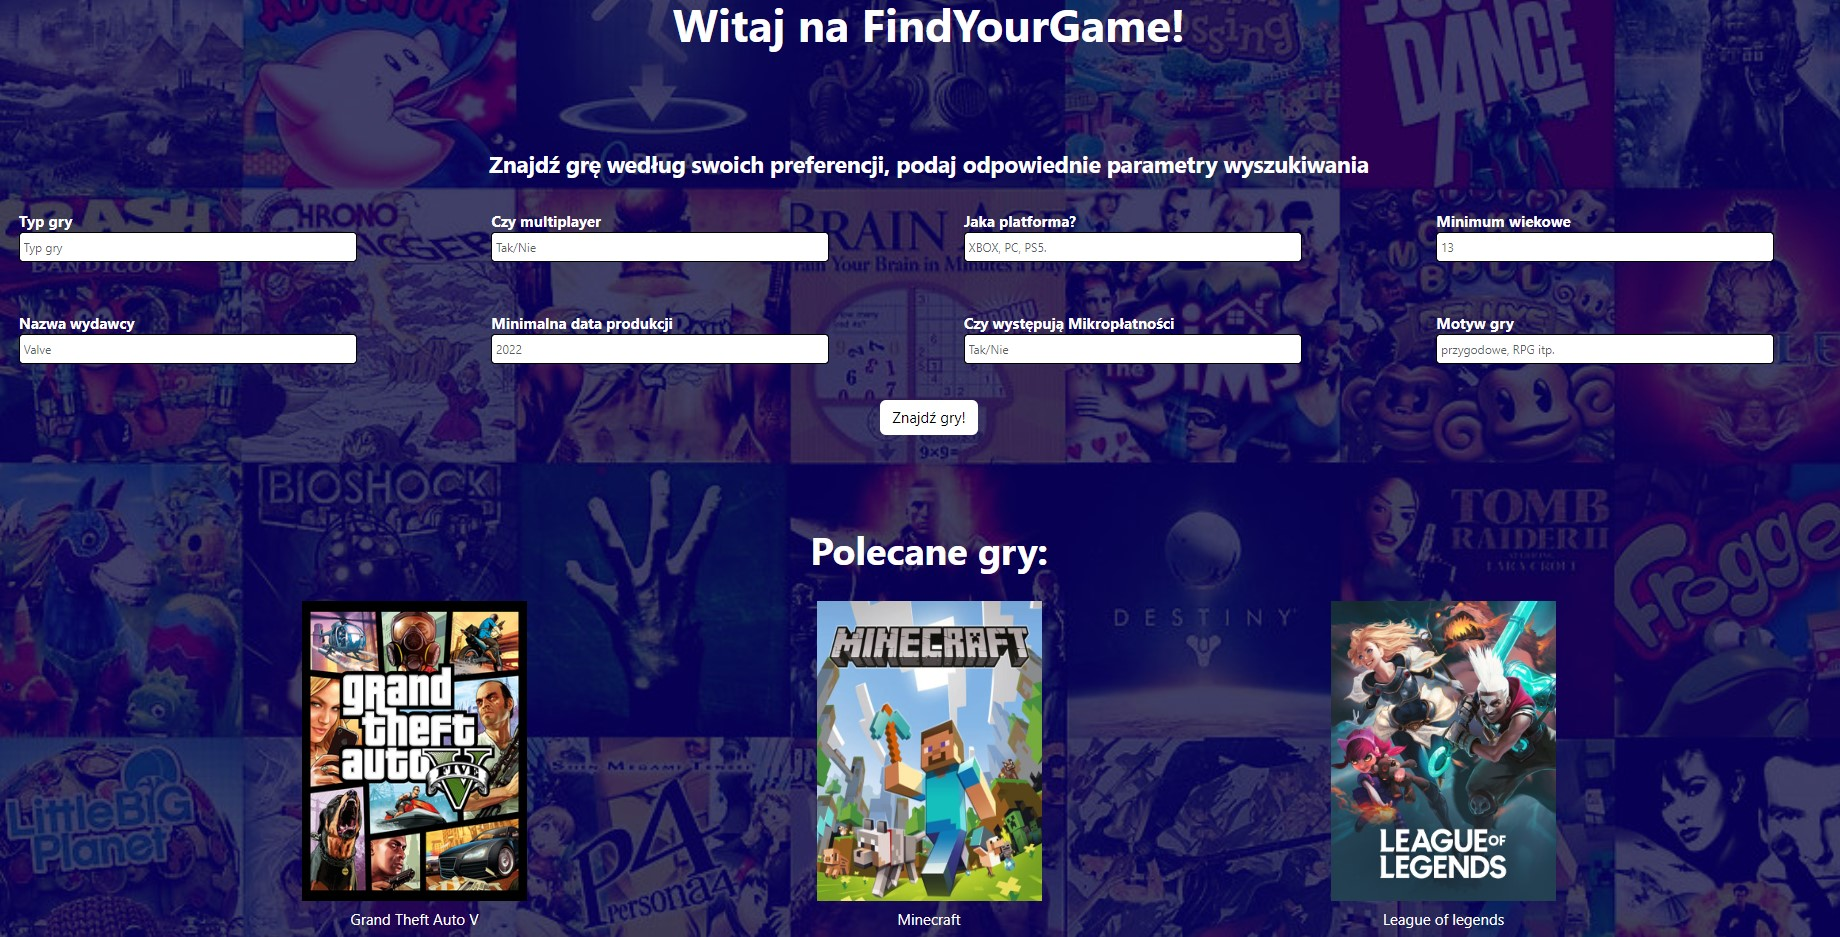
\includegraphics[width=1\linewidth]{./img/stronaglowna.jpg}
    \caption{Strona główna aplikacji}
    \label{fig:StronaGlowna}
\end{figure}

Na stronie poza polami do wyszukiwania, widzimy również polecane gry przez innych użytkowników. 
Użytkownik może wprowadzić 8 parametrów do wyszukiwania gry takich jak:
\begin{itemize}
\item \textbf{Typ gry:} np. RPG, FPS, Adventure, Strategy, MOBA, Sports, Racing
\item \textbf{Czy multiplayer:} pole powinno przyjmować wartości Tak lub Nie w zależności od tego na jakiej grze nam zależy
\item \textbf{Jaka platforma:} np. PC, XBOX One, XBOX Series X, PlayStation 4, Playstation 5, Google, Nintendo, VR, Steam
\item \textbf{Minimum wiekowe:} pole określa wiek gry licząc datę teraźniejszą odjąć data wydania gry
\item \textbf{Nazwa wydawcy:} np. Electronic Arts, Ubisoft, Nintendo, Rockstar Games
\item \textbf{Minimalna data produkcji:} pole określa rok wydania minimalny dla gry. Jeśli gra została wydana wcześniej niż podano, nie zostanie wzięta pod uwagę
\item \textbf{Czy występują Mikropłatności:} pole typu Tak/Nie
\item \textbf{Motyw gry:} np: Apocalypse, Medieval, Space, Cyberpunk, Pirates, Western
\end{itemize}
Po wprowadzeniu parametrów w całości lub częściowo, użytkownik powinien kliknąć przycisk \textit{Znajdź grę}.
Kod dla przycisku:
\begin{lstlisting}
          <div class="button-container">
            <button class="btn btn-lg">Znajdź gry!</button>
          </div>
\end{lstlisting}
Obsługa po kliknięciu:
\begin{lstlisting}
  submitGameForm():void {
    console.log(this.gameForm.value)
    const formData = this.gameForm.value;

    this.http.post<Game[]>('http://localhost:8080/api/games/findByCriteria', formData).subscribe(
      (response) => {
        this.games = response;
        this.gameService.setGames(this.games);
        console.log(this.games);
        this.router.navigate(['/secondpage']);
      },
      (error) => {
        console.error('Error:', error);
      }
    );
  }
\end{lstlisting}
Po wciśnięciu przycisku aplikacja frontendowa, woła endpoint wystawiony z aplikacji backendowej wyszukując odpowiednie gry dla zadanych parametrów. To właśnie w tym momencie zapisujemy wynik mierzenia czasu pobierania danych z baz Oracle oraz Firebase. W przypadku braku gier, lista parametrów jest sukcesywnie skracana o kolejne parametry, aby znaleźć minimum 3 gry do wyświetlenia.

Po znalezieniu gier użytkownik zostaje przeniesiony na drugą stronę, na której znajduje się karuzela z 3 grami dopasowanymi do jego preferencji oraz przyciski do potwierdzenia lub odrzucenia dopasowania tej gry:
\begin{figure}[h]
    \centering
    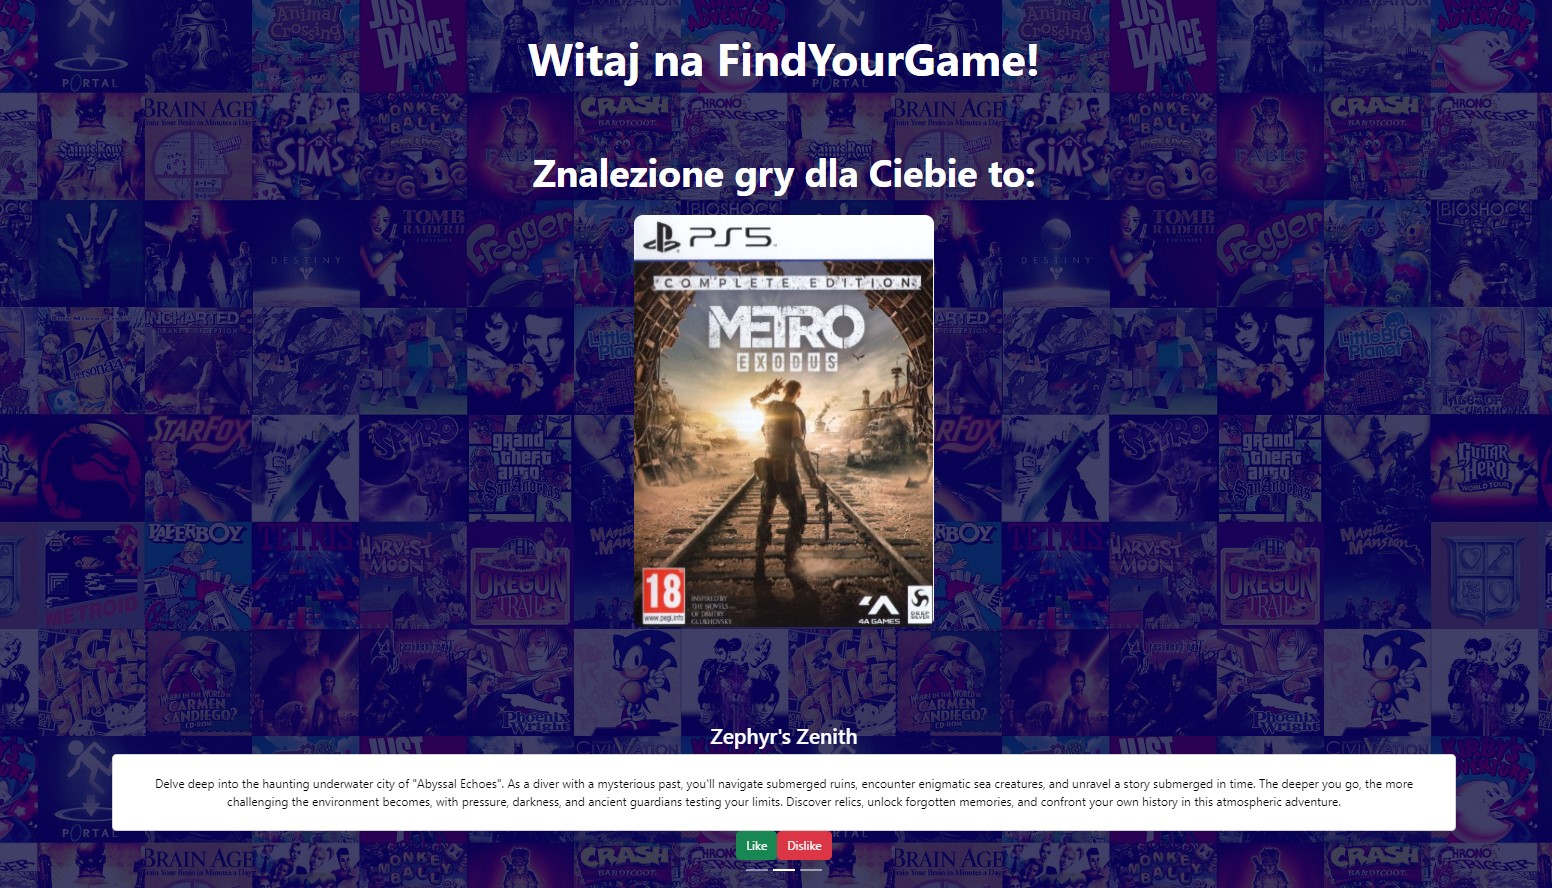
\includegraphics[width=1\linewidth]{./img/secondpage.jpg}
    \caption{Strona z wynikiem wyszukiwania}
    \label{fig:StronaWynik}
\end{figure}
Po wybraniu przycisku \textit{Like} lub \textit{Dislike}, przyciski znikają aby ograniczyć nadmierne głosy użytkowników.